\documentclass{article}
\usepackage{amsmath}
\usepackage{amssymb}
\usepackage{tikz}
\usepackage[utf8]{inputenc}
\usepackage{fontspec} % This line only for XeLaTeX and LuaLaTeX
\usepackage{pgfplots}
\usepgfplotslibrary{groupplots}
\pgfplotsset{compat=1.13}
\usepackage[hidelinks]{hyperref}
\usepackage{standalone}

\title{Complex gated memory cells.}
\author{Moritz Wolter  \\
    Uni Bonn  \\
    \and 
    Angela Yao \\
    Uni Bonn \\
    }

\date{\today}
% Hint: \title{what ever}, \author{who care} and \date{when ever} could stand 
% before or after the \begin{document} command 
% BUT the \maketitle command MUST come AFTER the \begin{document} command! 
\begin{document}
\tableofcontents
\newpage
\maketitle
\begin{abstract}
RNN optimization often suffers from numberically unstable gradients. We propose a novel complex RNN architecture, which can be shown to be numerically stable. Building on top of recent sucesses in the optimization of complex valued neural networks we propose a novel memory cell, which allows us to take gated recurrent units to the complex domain. In short we optimize: 
\begin{align}
\min_{\mathbf{W}} \text{cost}(\{\mathbf{x}\}, \{\mathbf{W}\}) \\
\text{such that } \forall m \; \| \phi_m \| = 1, \\
                  \forall n \; \| f'(h_n) \| \leq 1.
\end{align}
Where $\{\mathbf{W}\}$ denotes the set of network weights $\{\mathbf{x}\}$ the set of network inputs and $\{\phi_m\}$ the set of all weight matrix eigenvalues and finally $\|f'(h_n) \|$ the hidden actication derivatives.
We show that our complex gated memory cells are practically stable and use wirtinger calculus to overcome limitations on skalar activations set by Liouville's theorem. It turns out that we do not need to work with a constrained optimization algorithm here, but can instead rewrite the problem in an unconstrained way, and use libraries optimized for large scale unconstrained optimization such as tensorflow or pytorch.
\end{abstract}

\section{Introduction}
The training process of artificial neural networks is not necessarily stable. Unstable problem formulations lead to problems which are hard to optimize and converge slowly. Recently \cite{Arjovsky} has been able to prove that recurrent neural networks with normalized eigenvalues and bounded activiation derivatives must be stable. 

\section{Related work}
Normalized complex matrices where first introduced into the literature by \cite{Arjovsky}. Since then \cite{Wisdom}, expanded the reach of the unitary matrix basis. An idea that is taken further by \cite{Hyland}, which makes use Lie group theory.  
A holomorph non-linearity was used in \cite{Guberman}, \cite{Arjovsky} introduces a novel non-linearity which is not complex-differentiable. \cite{Trabelsi} compares complex non-linearities and systematically measures performance. Furthermore complex batch-normalization is introduced.
Finally \cite{Jing}, proposes a gated unitary RNN, but is restricted to the real numbers. \\
Finding a gradient for functions from $\mathbb{C}$ to $\mathbb{R}$, is a problem which has been adressed in the digital signal processing literature. Where complex problems with real cost functions had to be solved \cite{Brandwood}\cite{Bos}\cite{Franken}\cite{Delgado}. Applications to neural network cost functions where considered later \cite{Mandic}. All solutions essentially utilize Wirtinger calculus \cite{Wirtinger}, to come up with an approximate gradient for a non-holomorph function.

\section{Complex Unitary Memory cells}
Setting up complex gating mechanisms is no trivial task, because functions from $\mathbb{C} \rightarrow \mathbb{R}$ cannot be holomorph unless they are constant \cite[page 9]{Bornemann}\footnote{Proof: \url{https://math.stackexchange.com/questions/1004672/prove-that-a-real-valued-constant-function-is-holomorphic-and-vice-versa}}. Furthermore bounded holomorph complex functions must be constant \cite[page 38]{Bornemann}\footnote{\url{https://en.wikipedia.org/wiki/Liouville\%27s\_theorem\_(complex\_analysis)}}.
Classic multiplication gates with $0 \leq |f(x)| \leq 1$ and $\mathbb{C} \rightarrow \mathbb{R}$ which rely on $f(x) \cdot h$ are therefore hard to implement, because there is no obvious complex gradient to train these gates. 
We define:
\begin{align}
\mathbf{i}_g &= \sigma(\mathbf{U}_i[\Re(\mathbf{h}_t) \; \Im(\mathbf{h}_t)]^T
                + \mathbf{W}_i[\Re(\mathbf{x}) \; \Im(\mathbf{x})]^T )\\
\mathbf{f}_g &= \sigma(\mathbf{U}_f[\Re(\mathbf{h}_t) \; \Im(\mathbf{h}_t)]^T
                + \mathbf{W}_f[\Re(\mathbf{x}) \; \Im(\mathbf{x})]^T )\\
\mathbf{h}_{t+1} &= \mathbf{U}f(\mathbf{f}_g \odot \mathbf{h}_t) + \mathbf{W}(\mathbf{i}_g \odot \mathbf{x})
\end{align}
Where $\mathbf{U}$ is a unitary matrix and $\mathbf{i}_g, \mathbf{f}_g$ are computed by mappings from $\mathbb{C} \rightarrow \mathbb{R}$. Our gates are therefore non-holomorph. We leverage Wirtinger calculus \cite{Franken}\cite{Delgado}\cite{Wirtinger}, to define a pseudogradient, which we argue is sufficient to train the gates. Please note that we do not distribute our derivatives over a sum, a major difference to the classical formulation in \cite{Hochreiter}. \\ 
\textit{TODO: explain our gradient approximation.}

\subsection{Proof of stability}
Hochreiter et al. \cite{Hochreiter} have shown, that a similar cell defined on $\mathbb{R}$, must be stable. Following \cite{Arjovsky} we prove that Complex Unitary Memory cells are also be stable:
\begin{align}
\frac{\partial C}{\partial h_{t}} &= \frac{\partial C}{\partial h_T}\frac{\partial h_T}{\partial h_t} \\
                                  &= \frac{\partial C}{\partial h_T}\prod_{k=t}^{T-1}\frac{\partial h_{k+1}}{\partial h_k} \\
                                  &= \frac{\partial C}{\partial h_T}\prod_{k=t}^{T-1}\mathbf{U}
                                  \mathbf{G}_{k+1} \frac{\partial \text{f}}{\partial h_k}
\end{align}

\subsection{Results}
\begin{figure}
\centering
%\includestandalone[width=0.45\linewidth]{./img/cgmu/adding_problem}
\includegraphics[width=0.45\linewidth]{./img/cgmu/adding_problem.pdf}
%\includestandalone[width=0.45\linewidth]{./img/cgmu/memory_problem}
\includegraphics[width=0.45\linewidth]{./img/cgmu/memory_problem.pdf}
\caption{Performance of the complex gated memory unit (cgmu, ours), the unitary neural network (unn, \cite{Arjovsky}), and long short term memory (lstm, \cite{Hochreiter}).}
\label{fig:montreal_eval}
\end{figure}
To test our ideas we used the benchmark originally proposed in \cite{Hochreiter} following the implementation of \cite{Arjovsky}. A visualization of our results is shown in figure~\ref{fig:montreal_eval}. All modes where run with a state size of $512$, step size of $0.001$ and a batch size of $250$. For the memory problem, the baseline is at $0.173$, which all models beat. For the adding problem it is $0.167$. Again all models crack this treshhold. However the convergence behaviour differes. We argue that our apprach gets the bost of both worlds in terms of performance an converges well on both the adding and memory problems, it shows the supereor UNN dynamics on the memory problem, while at the same time behaving more like the LSTM on the adding problem, where it significantly outperforms both other models.

\section{Other Ideas}
\subsection{Fourier Space rotations.}
Earlier work has found that rotations can be implemented in the frequency domain by shearing along 
the two dimensions. Making use of the DFTs shift theorem \cite[page 173]{Briggs}:\footnote{\url{http://www.nontrivialzeros.net/KGL_Papers/27_Rotation_Paper_1997_qualityscan_OCR.pdf}}
\footnote{\url{http://bigwww.epfl.ch/publications/unser9502.pdf}}
\begin{align}
\mathcal{D}(f_{m + m_0, n + n_0}) = \omega_M^{-m_0j}\omega_N^{-n_0k}F_{jk} \\
\text{with } \omega_N^{nk} = e^{i2\pi nk/N}
\end{align}
Transformation to the frequency domain multiplication, rotation and inverse transformation, can be implemented using three matrix multiplications, when working with the DFT or as FFT, multiplication and ifft. The inverse transformation is a way to implicitly apply trigonometric interpolation\footnote{\url{https://en.wikipedia.org/wiki/Trigonometric_interpolation}}. Which takes care of interpolating the pixel values of the new rotated image.

Some first numerical evidence suggests that fourier rotation matrices are unitary. This could allow us to prove stability. TODO: Proof?

\subsection{Unitary dynamic filter networks}
Motivation: Current dynamic RNNs do not worry about stability. \\
Idea: Adapt RNN stability theory to come up with stable dynamic RNNs. \\
Extra motivation: I think that the steerable filter paper \cite{Freeman} was the basis for the original dynamic filter paper. Which is why I think the fourier extension of this paper \cite{Michaelis} could hold some cues for a nice extension. In particular, because outside of the vision domain, \cite{Hyland} has already shown that this is an interesting idea. 

\section{Background}

\subsection{Phase-Relus}
Holomorph functions $f(x,y) = u(x,y) + iv(x,y)$ must satisfy the Cauchy-Riemann equations:
\begin{align}
\frac{\partial u}{\partial x} = \frac{\partial u}{\partial y} \; \text{and} \; \frac{\partial u}{\partial y} = -\frac{\partial v}{\partial x}  
\end{align}
This form has been considered in \cite{Trabelsi} and used to evalute existing non-linearities such as the zRelu, cRelu or Mod-Relu. However we believe it is much more intuitive to consider the Cauchy-Riemann equations in polar form \footnote{Proof see: \url{https://math.stackexchange.com/
questions/1245754/cauchy-riemann-equations-in-polar-form}}:
\begin{align}
\frac{\partial u}{\partial r} = \frac{1}{r} \frac{\partial v}{\partial \theta} \; \text{and} \; \frac{\partial v}{\partial r} = - \frac{1}{r} \frac{\partial u}{\partial \theta}
\end{align}
Which allows us to design a non-linearity using $z = re^{i\theta}$ and $f(r,\theta ) = u(r,\theta ) + iv(r,\theta )$. We will focus on non-linearities of the form:
\begin{align}
f(r, \theta) &= g(r,\theta,a,b) e^{i \theta} \\
&= g(r,\theta,a,b)\cos(\theta) + ig(r,\theta,a,b)\sin(\theta)
\end{align}
With $a,b$ as lernable function parameters. Setting $g(r,\theta,a,b)$ to:
\begin{align}
g(r,\theta,a,b) = r \text{H}(\sin (\theta \cdot a\pi + b))
\label{eq:PhaseRelu}
\end{align}
With H denoting the Heaviside step function and $a,b \in \mathbb{R}$.
\begin{figure}
    \centering
    \includestandalone{image-code/sine_step}
    \includestandalone{image-code/shifted_sine_step}
    \caption{Plot of the $\sin(\theta a\pi + b\pi)$ and $\text{H}(\sin(\theta a\pi + b\pi))$ with $a=1, b=0$ (left) and $a=2, b=0.1$}
    \label{fig:step_sine}
\end{figure}
Leads to the conditions:
\begin{align}
\frac{\partial u}{\partial r} &= \text{H}(\sin (\theta \cdot a\pi + b)) \cos \theta, \\ 
\frac{\partial v}{\partial r} &= \text{H}(\sin (\theta \cdot a\pi + b)) \sin \theta, \\
\frac{\partial u}{\partial \theta} &= -r \text{H}(\sin (\theta \cdot a\pi + b)) \sin \theta \nonumber \\
&\quad + r \delta(\sin (\theta \cdot a\pi + b)) \cos(\theta \cdot a\pi + b))a\pi \cos(\theta)\\ 
\frac{\partial v}{\partial \theta} &= r \text{H}(\sin (\theta \cdot a\pi + b)) \cos \theta \nonumber \\
&\quad + r \delta(\sin (\theta \cdot a\pi + b)) \cos(\theta \cdot a\pi + b))a\pi \sin(\theta)
\end{align}
Above $\delta$ denotes Dirac's distribution, which we consider to be zero for all practical purposes. 
We therefore argue that this non-linearity which we call Polar-Relu is approximately holomorph\footnote{Strictly speaking it is holomorph, when excluding all points where $\sin (\theta \cdot a\pi + b)$ = 0.}.\\
$\text{H}(\sin(\theta \cdot a \pi + b)$ sets the output to zero, whenever $\sin (\theta \cdot a\pi + b) < 0$. We must have $\theta \in [0, 2\pi]$. This means for $a = 1, b = 0$ this non-linearity removes the lower-half of the complex plane with $\theta > \pi$ where $\Re(z) < 0$. When keeping $b=0$, for $0.5 < |a| < 1$ the filtered spectrum is reduced, and for $|a| < 0.5$, no values are filtered. Working with $|a| > 1$ introduces periodically spaced smaller filters. Because the sine wave will complete more than one iteration for $\theta$. Finally $b$ rotates the filter around the origin, this parameter enables layered phase relus to individually remove different areas of the complex plane. \\
An interesting variant of this approach can be created by adding a cosine term to equation~\ref{eq:PhaseRelu}:
\begin{align}
g(r,\theta,a,b,c,d) = r \text{H}(\sin (\theta \cdot a\pi + b))\text{H}(\cos (\theta \cdot c\pi + d))
\end{align}
This will kill any incoming complex number with a phase angle of either zero sine or cosine. The above equation can be considered a generalization of the zRelu from \cite{Guberman}\cite{Trabelsi}. Its is equivalent for $a=1, b=0, c=1, d=0$ because both cosine and sine are positive in the first quadrant. This approach works when choosing the function parameters manually. Unfortunately, the same mechanics, that makes this approach approximately holomorph also kills the derivative, which one would want to use to train the function parameters.  \\

\subsubsection{Phase-Relu approximate stability proof in Cartesian coordinates.}
\label{sec:CarthesianPhaseRelu}
We have shown that 
\begin{align}
f(r,\theta) = r\text{H}\sin(\theta \cdot a \pi + b)e^{i\theta}
\end{align}
is stable in polar coordinates. For the extremely skeptical reader we will now show that its equivalent form:
\begin{align}
f(x + iy) = \text{H}(\sin(\text{atan2}(x,y)))(x + iy)
\end{align}
is stable in Cartesian coordinates.
Splitting the above formulation into real and imaginary parts leads to:
\begin{align}
f(x + iy) = x\text{H}(\sin(\text{atan2}(x,y))) + i y\text{H}(\sin(\text{atan2}(y/x)))
\end{align} 
We recognize the form $f(z) = u + iv$. Working with the unchanged Cauchy-Riemann equations:
\begin{align}
\frac{\partial u}{\partial x} = \frac{\partial v}{\partial y}, \;\;\; \frac{\partial u}{\partial y} = - \frac{\partial v}{\partial x},
\end{align}
and using the facts that the derivatives of $\text{atan2}(x,y)$ are equal to those of $\tan^{-1}(y/x)$ which are $\frac{\partial \tan^{-1}(y/x)}{\partial x} = -\frac{y}{x^2 + y^2}$ and $\frac{\partial \tan^{-1}(y/x)}{\partial y} = \frac{x}{x^2 + y^2}$, we derive:
\begin{align}
\frac{\partial u}{\partial x} &= \text{H}(\sin(\tan^{-1}(y/x))) \nonumber \\
&\quad +x\delta(\sin(\text{tan}^{-1}(y/x)))\cos(\tan^{-1}(y/x))(\frac{-y}{x^2 + y^2})(\frac{-y}{x^2}) \\
\frac{\partial u}{\partial y} &= \delta(\sin(\tan^{-1}( y/x)))\cos(\tan^{-1}(y/x))(\frac{x}{x^2 + y^2}) \\
\frac{\partial v}{\partial x} &= y\delta(\sin(\tan^{-1}( y/x)))\cos(\tan^{-1}(y/x))(\frac{-y}{x^2 + y^2})(\frac{-y}{x^2}) \\
\frac{\partial v}{\partial y} &= \text{H}(\sin(\tan^{-1}(y/x))) \nonumber \\
&\quad + y\delta(\sin(\text{tan}^{-1}(y/x)))\cos(\tan^{-1}(y/x))(\frac{x}{x^2 + y^2})(\frac{1}{x})
\end{align}
Most of the time the Dirac terms $\delta(\cdot)$ will be zero and $\frac{\partial u}{\partial x} = \frac{\partial v}{\partial y} = \text{H}(\sin(\tan^{-1}(y/x)))$ as well as $\frac{\partial u}{\partial y} = - \frac{\partial v}{\partial x} = 0$ will hold. The derivative is zero if the non-linearity is inactive and 1 when its active and therefore bounded.


\subsection{Analysis of existing complex activation functions.}
This section is dedicated to the analysis of previously proposed non-linearities and relies on using the Cauchy-Riemann equations given by:
\begin{align}
\frac{\partial u}{\partial x} = \frac{\partial v}{\partial y}, \;\;\; \frac{\partial u}{\partial y} = - \frac{\partial v}{\partial x},
\end{align}
for $f(z) = u(x,y) + iv(x,y)$ or if $f(r, \theta) = u(r, \theta) + iv(r, \theta)$, we make use of:
\begin{align}
\frac{\partial u}{\partial r} = \frac{1}{r} \frac{\partial v}{\partial \theta} \; \text{and} \; \frac{\partial v}{\partial r} = - \frac{1}{r} \frac{\partial u}{\partial \theta}
\end{align}
which is equivalent.
\subsubsection{zRelu}
\begin{align}
\text{zRelu}(z) =\begin{cases} z \text{ if } \theta \in [0, \pi/2], \\
                               0 \text{  else}.
                 \end{cases}
\end{align}
Following \cite{Trabelsi} we have for the first quadrant:
\begin{align}
\frac{\partial u}{\partial x} = \frac{\partial v}{\partial y} = 1,\\
\frac{\partial u}{\partial y} = -\frac{\partial v}{\partial x} = 0, 
\end{align}
and elsewhere:
\begin{align}
\frac{\partial u}{\partial x} = \frac{\partial v}{\partial y} = 0,\\
\frac{\partial u}{\partial y} = -\frac{\partial v}{\partial x} = 0,
\end{align}
holds. On the real and imaginary axes, the two areas are not smoothly connected, which is why we must include them. This argument may be backed up by considering the equivalent Phase-Relu formulation as defined in section~\ref{sec:CarthesianPhaseRelu}:
\begin{align}
\text{zRelu}(z) = \text{H}(\sin(\text{atan2}(x,y)))\text{H}(\cos(\text{atan2}(x,y)))(x + iy)
\end{align}
Which is an equivalent way to write the zRelu, its Dirac pulse derivatives are one on the real and imaginary axis, which is why the this non-linearity is not holomorph there. The derivative is either zero or one and therefore bounded. These desirable properties come at the cost of having to throw away three quarters of the complex plane, which seems unnecessarily wasteful.

\subsubsection{modRelu}
\label{sec:modRelu}
The modRelu is defined as \cite{Arjovsky}:
\begin{align}
f(z) = \text{Relu}(\|z\| + b) \frac{z}{\|z\|}.
\end{align}
Conversion to polar coordinates yields:
\begin{align}
f(r, \theta) &= \text{Relu}(r + b)e^{i\theta}, \\
f(r, \theta) &= \text{Relu}(r + b)\cos(\theta) + i\text{Relu}(r + b)\sin(\theta). \\
\end{align}
we find $u(r, \theta) = \text{Relu}(r + b)\cos(\theta)$ and $v(r, \theta) = \text{Relu}(r + b)\sin(\theta)$. The polar Cauchy-Riemann equations yield:
\begin{align}
\frac{\partial u}{\partial r} &= \text{H}(r + b)\cos(\theta),  \\
\frac{\partial u}{\partial \theta} &= -\text{Relu}(r + b)\sin(\theta), \\
\frac{\partial v}{\partial r} &= \text{H}(r + b)\sin(\theta), \\
\frac{\partial v}{\partial \theta} &= \text{Relu}(r + b)\cos(\theta).
\end{align}
For holomorphy we require:
\begin{align}
\frac{\partial u}{\partial r} &= \frac{1}{r} \frac{\partial v}{\partial \theta}, \\
\Leftrightarrow r\text{H}(r + b)\cos(\theta) &= \text{Relu}(r + b)\cos(\theta);\\
\frac{\partial v}{\partial r} &= - \frac{1}{r} \frac{\partial u}{\partial \theta}, \\ 
\Leftrightarrow r\text{H}(r + b)\sin(\theta) &= \text{Relu}(r + b)\sin(\theta).
\end{align}
Taking into account the fact that $r\text{H}(r) = \text{Relu}(r)$ we have $r\text{H}(r + b) \approx \text{Relu}(r + b)$ if $b \approx 0$. The modRelu non-linearity is therefore only holomorph when it is approximately linear, not a useful property. Furthermore we find:
\begin{equation}
\frac{\partial}{\partial z}\sigma_{\text{Relu}}(\|z\| + b) \frac{z}{\|z\|} = \sigma_{\text{Relu}}'(\|z\| + b) \frac{z}{\|z\|} + \sigma_{\text{Relu}}(\|z\| + b) (\frac{z}{\|z\|})'.
\end{equation}
By applying the product rule. The left part of the resulting sum is stable, but the right part is not bounded and therefore unstable, which is yet another undesirable property.

\subsubsection{cRelu}
\cite{Trabelsi} defines the cRelu as:
\begin{align}
\text{cRelu}(z) = \text{Relu}(x) + i\cdot \text{Relu}(y).
\end{align}
Thus $u = \text{Relu}(x)$ and $v = \text{Relu}(y)$.
In the first quadrant we have:
\begin{align}
\frac{\partial u}{\partial x} = \frac{\partial v}{\partial y} = 1,\\
\frac{\partial u}{\partial y} = -\frac{\partial v}{\partial x} = 0.
\end{align}
For the second we find:
\begin{align}
\frac{\partial u}{\partial x} = 0 \neq \frac{\partial v}{\partial y} = 1,\\
\frac{\partial u}{\partial y} = -\frac{\partial v}{\partial x} = 0, 
\end{align}
The third quadrant has:
\begin{align}
\frac{\partial u}{\partial x} = \frac{\partial v}{\partial y} = 0,\\
\frac{\partial u}{\partial y} = -\frac{\partial v}{\partial x} = 0, 
\end{align}
Finally considering the fourth:
\begin{align}
\frac{\partial u}{\partial x} = 1 \neq \frac{\partial v}{\partial y} = 0,\\
\frac{\partial u}{\partial y} = -\frac{\partial v}{\partial x} = 0, 
\end{align}
In its holomorph region the derivative of the function is one just like in the real case which is stable.
We have shown this definition to be holomorph when $\text{sign}(\Re(z)) = \text{sign}(\Im(z))$\cite{Trabelsi}, which is the case in the first an third quadrant. When restricting this definition to the first quadrant and setting it to zero elsewhere, one obtains the $\text{zRelu}$ which is a holomorph function. \\

\subsubsection{Cardioid}
\cite{Virtue} introduces the complex cardioid,:
\begin{align}
f(z) = \frac{1}{2}(1 + cos(\theta))z
\end{align}
Which we express in polar-coordinates as:
\begin{align}
f(r, \theta) = \frac{1}{2}(1 + cos(\theta))re^{i\theta}
\end{align}
Using the definition of the complex exponential we obtain:
\begin{align}
f(r, \theta) = \frac{1}{2}(1 + cos(\theta))r\cos(\theta) + i\frac{1}{2}(1 + cos(\theta))r\sin(\theta) 
\end{align}
Reading of $u = \frac{1}{2}(1 + cos(\theta))r\cos(\theta)$ and $v = \frac{1}{2}(1 + cos(\theta))r\sin(\theta)$ we find:
\begin{align}
\frac{\partial u}{\partial r} &= \frac{1}{2}(1 + \cos(\theta))\cos(\theta) \\
\frac{\partial u}{\partial \theta} &= -r\frac{1}{2}(1 + \cos(\theta))\sin(\theta) - r\frac{1}{2}\sin(\theta)\cos(\theta) \\
\frac{\partial v}{\partial r} &= \frac{1}{2}(1 + \cos(\theta))\sin(\theta) \\
\frac{\partial v}{\partial \theta} &= r\frac{1}{2}(1 + \cos(\theta))\cos(\theta)) - r\frac{1}{2}\sin(\theta)\cos(\theta)
\end{align}
And therefore we require:
\begin{align}
\frac{\partial u}{\partial r} = \frac{1}{2}(1 + \cos(\theta))\cos(\theta) &= \frac{\partial v}{r\partial \theta} =  \frac{1}{2}(1 + \cos(\theta)\cos(\theta)) - r\frac{1}{2}\sin(\theta)\cos(\theta) \\
\Leftrightarrow 0  &= - r\frac{1}{2}\sin(\theta)\cos(\theta) \\
\end{align}
Which is holomorph at $r=0$. When $r \neq 0$ excluding everything except for the real and imaginary axes is necessary, there the trigonometric functions are zero. Where the derivative exists it is unstable when $\cos(\theta) > 0$, which happens if $0 \leq \theta < \pi/2$ and $3/2\pi < \theta \leq 2\pi$. This is the case on the real axis where $\theta = 0$. In other words the Cardioid has a defined and stable derivative only on the imaginary axis.

\subsubsection{Phase-amplitude activation}
\cite{Scardapane} cites these as:
\begin{align}
f(z) = \tanh(r/m)e^{i\theta}
\end{align}
Considering the polar C.R. equations:
\begin{align}
f(r,\theta) &= \cos(\theta)\tan^{-1}(r/m) + i\sin(\theta)\tan^{-1}(r/m) \\
            &\Rightarrow u + iv \nonumber \\
\frac{\partial u}{\partial r} &= \cos(\theta)\text{sech}^2(r/m)(1/m) \\
\frac{\partial u}{\partial \theta} &= -\sin(\theta)\tanh(r/m) \\
\frac{\partial v}{\partial r} &= \sin(\theta)\text{sech}^2(r/m)(1/m) \\
\frac{\partial v}{\partial \theta} &= \cos(\theta)\tanh(r/m) \\
\Rightarrow  \frac{\partial u}{\partial r} &=\frac{\partial v}{r\partial \theta} \nonumber \\
\Leftrightarrow \qquad & \cos(\theta)\text{sech}^2(r/m)(1/m) = \frac{1}{r}\cos(\theta)\tanh(r/m) \\
\Leftrightarrow \qquad & \text{sech}^2(r/m)(r/m) = \tanh(r/m)
\label{eq:holo-pa}
\end{align}
\begin{figure}
\centering
\includegraphics{./img/phase_amplitude_cond.pdf}
\caption{Plot of the holomorphy condition's two sides for the Phase-amplitude activation. $\tanh(r/m)$ is shown in red, $\text{sech}^2(r/m)(r/m)$ is shown in blue. The yellow circle indicates the point at $(0,0)$.}
\label{fig:phase_amp}
\end{figure}
This activation is holomorph at $r/m = 0$. And approximately analytic for $r/m \approx 0$ as shown in figure~\ref{fig:phase_amp}, the problem here is that this non-linearity breaks magnitude information by rescaling them, it must therefore be non-holomorph for large inputs. 

\subsection{Backward mode automatic differentiation gradients}
Consider the non-linear network proposed in \cite{Pascanu}:
\begin{align}
\mathbf{x}_t  = W_{\text{rec}}f(\mathbf{x}_{t-1}) + W_{\text{in}}\mathbf{u}_t + \textbf{b}
\end{align}
Following \cite{Pascanu} we define the error function $\mathcal{E}_t = \mathcal{L}$ and work with BPTT gradients given by:
\begin{align}
\frac{\partial \mathcal{E}}{\partial \theta} &= \sum_{1 \leq t \leq T} \frac{\mathcal{E}_t}{\partial \theta} \\
\frac{\partial\mathcal{E}_t}{\partial\theta} &= \sum_{1 \leq k \leq t}( \frac{\mathcal{E}_t}{\partial \mathbf{x}_t} \frac{\partial \mathbf{x}_t}{ \mathbf{x}_k} \frac{\partial^+ \mathbf{x}_k}{\partial \theta}) \label{eq:gradsum}\\
\frac{\partial \mathbf{x}_t}{ \partial \mathbf{x}_k} &= \prod_{t \geq i > k} \frac{\partial \mathbf{x}_i}{ \partial \mathbf{x}_{i-1}} = \prod_{t \geq i > k} W^T_{\text{rec}} \text{diag}(f'(\mathbf{x}_{i-1}))
\end{align}
The above equations are essential a consistent application of the chain rule. It is important to note that $\partial^+ \mathbf{x}_{k} / \partial W_\text{rec} = f(\mathbf{x}_{k-1})$.

\subsubsection{The linear case}
Working with $f(x) = x$ according the long term behavior is determined by the matrix product $\partial \mathbf{x}_t / \partial \mathbf{x}_k$ \cite{Pascanu}. We define $W_{\text{rec}} = C$, and normalize the spectrum of C to $\forall k \; \| \phi_k \| = 1$ for $k \in \{1 \dots n\}$. Focusing on the term in the sum of equation~\ref{eq:gradsum}, we express $\partial \mathcal{E} / \partial \mathbf{x}_t $ in terms of a Fourier basis:
\begin{align}
\frac{\partial \mathcal{E}}{\partial \mathbf{x}_t} = \sum_{i=1}^n \mathbf{f}_i^T d_i  
\end{align}
Knowing the Fourier vectors are eigenvectors of $C$, which leads to $\mathbf{f}_i^T(C^T)^l = \phi_i^l\mathbf{f}_i^T$ therefore we have:
\begin{align}
\frac{\partial \mathcal{E}}{\partial \mathbf{x}_t}\frac{\partial \mathbf{x}_t}{\partial \mathbf{x}_k} = 
\sum_{i=1}^n \mathbf{f}_i^T d_i \phi_i 
\end{align}
Having chosen $\| \phi_k \| = 1$, we can approximate:
\begin{align}
\frac{\partial \mathcal{E}}{\partial \mathbf{x}_t}\frac{\partial \mathbf{x}_t}{\partial \mathbf{x}_k} = 
\sum_{i=1}^n \mathbf{f}_i^T d_i \phi_i 
\approx \sum_{i=1}^n \mathbf{f}_i^T d_i =\frac{\partial \mathcal{E}}{\partial \mathbf{x}_t}
\end{align}
Because $\phi = \exp(i\omega)$ merely represents a rotation of the errors phase angle, but leaves its magnitude intact.
Using the train of tought borrowed from \cite{Pascanu}, we claim to establish an error carousel similar to Hochreiter 1998, through which errors can pass in a stable manner.

\subsubsection{Non-linear Cayley-Networks}
We could employ a non-linearity based on the Cayley-Transform \cite[p. 100]{Bornemann}:
\begin{equation}
C'(z) = \frac{z-i}{z+i}
\end{equation}
Which is guaranteed to map the upper half of the complex plane into the unit circle. Integrating $C(z)$
leads to;
\begin{equation}
C(z) = z - 2i\ln(z + i)
\end{equation}
Which leads to a possible non-linearity for $\Re(z) > 0$. The unstable lower part of the complex plane where $\Re(z) < 0$, could be removed by defining:
\begin{equation}
D'(z) = \frac{z+i}{z-i}
\end{equation}
And working with $D(z) = z + 2i\ln(z - i)$ where  $\Re(z) < 0$. Working with this definition all $z$ with $\Im(z) = 0$, would not be defined, because there is no smooth connection when crossing from $\Re(z) > 0$ to $\Re(z) < 0$ and the complex logarithm is not defined for all $\Re(z) < 0$ with $\Im(z) = 0$.
Cayley transforms are known to be holomorph, which is a general property of all Möbius transforms.


\subsection{Convolutions and circulant matrices}
One dimensional convolutions can be expressed as multiplication with a circulant matrix.
The convolution operations used in neural networks may be expressed as matrix multiplication
with doubly circulant matrices \cite[page 324]{goodfellow}, doubly referring to a circulant block matrix consisting of circulant blocks. 
The eigen-decompositions of both cases seem to be well understood in the specialized mathematical literature\footnote{\url{http://nzjm.math.auckland.ac.nz/images/8/8e/18-36.pdf}}.

\subsection{1D-convolutions and circulant matrices}
\begin{figure}
\centering
\begin{minipage}{.45\textwidth}
\begin{equation*}
C = \begin{pmatrix}
c_1 & c_2 & c_3 & c_4 \\
c_4 & c_1 & c_2 & c_3 \\
c_3 & c_4 & c_1 & c_2 \\
c_2 & c_3 & c_4 & c_1 \\
\end{pmatrix}
\end{equation*}
\end{minipage}
\begin{minipage}{.45\textwidth}
\scalebox{0.4}{% This file was created by matplotlib2tikz v0.6.15.
\begin{tikzpicture}

\begin{axis}[
hide x axis,
hide y axis,
xmin=-0.5, xmax=3.5,
ymin=-0.5, ymax=3.5,
tick align=outside,
tick pos=left,
x grid style={white!69.01960784313725!black},
y grid style={white!69.01960784313725!black}
]
\addplot graphics [includegraphics cmd=\pgfimage,xmin=-0.5, xmax=3.5, ymin=3.5, ymax=-0.5] {./img/circ1.png};
\addplot graphics [includegraphics cmd=\pgfimage,xmin=-0.5, xmax=3.5, ymin=3.5, ymax=-0.5] {./img/circ2.png};
\end{axis}

\end{tikzpicture}}
\end{minipage}
\caption{Circulant matrix structure as formula and in plotted form.}
\label{fig:circ1}
\end{figure}
Consider for example the four by four circulant matrix $C = circ(c_1,c_2,c_3,c_4)$
as shown in figure~\ref{fig:circ1}.
The matrix vector product $C\mathbf{x}$ with $\mathbf{x} = (x_1, x_2, x_3, x_4)^T$, can be written as:
\begin{align}
c_1x_1 + c_2x_2 + c_3x_3 + c_4x_4 \\
c_4x_1 + c_1x_2 + c_2x_3 + c_3x_4 \\
c_3x_1 + c_4x_2 + c_1x_3 + c_2x_4 \\
c_2x_1 + c_3x_2 + c_4x_3 + c_1x_4
\end{align}
Above one can nicely see how the kernel moves over the one dimensional signal in x. If the wrapping effect is not desired the edges of $x$ must be padded with zeros and parts of the circulant matrix be set to zero. For example $x_1, x_4 =0$ and $c_3,c_4=0$, will remove the wrap-around.

\subsection{The linear one-dimensional case}
According to \cite[page 33]{gray}, the eigenbasis of all circulant matrices is given by:
\begin{align}
\mathbf{f}^{(m)} = \dfrac{1}{\sqrt{n}}(1, \exp(-2\pi im/n), \dots, \exp(-2\pi im(n-1)/n))'
\end{align}
For all m eigenvectors. Given a set of complex eigenvalues $\{\phi_m\}$, the corresponding
circulant matrix can be computed using:
\begin{align}
C = F \Phi F^{-1}
\end{align}
For reasons which will become clear later we will express our eigenvalues in polar coordinates
as:
\begin{align}
\phi_m = r \exp{i\omega}
\end{align}
We propose the normalize network convolutions by setting their $r=1$ for all convolutions and all eigenvalues and optimize only the eigenangles $\omega$. Which amounts to requiring all
convolution matrices to have eigenvalues located on the unit circle or equivalently, we enforce 
$\| \phi_m \| = 1$. To construct $C$ we must transform all $\phi_m$s to Cartesian coordinates 
using $x_m= \cos(\omega)$ and $y_m=\sin(\omega)$. When then place the Cartesian eigenvalues $x_m + iy_m$ on the diagonal of $\Phi$. Next we can construct $C$ from $C = U \Phi U^{-1}$. Where $U$ is known and can be attached as a constant matrix to the computational graph. Furthermore the previous operations involve only trigonometric functions and matrix products, these operations are all differentiable, therefore we can find their gradient using standard AD tools.
By running the optimization in the $\omega$ space we can enforce $\| \phi_m \| = 1$, without having to work with a constrained optimization algorithm.

\subsection{Effects on linear network stability}
\subsubsection{Matrix power}   
\label{seq:linstab}
In this section we will evaluate the effect of $\| \phi_m \| = 1$ on a linear one dimensional bias-free convnet consisting of n layers.
\begin{align}
y &= C_1 \cdot C_2 \dots C_n \cdot x \\
y &= F \Phi_1 F^{-1} \cdot F\Phi_2 F^{-1} \dots \cdot F\Phi_n F^{-1} \cdot x \\
y &= F \Phi_1 \cdot \Phi_2 \dots \cdot \Phi_n F^{-1}\cdot x \\ 
\end{align}
All convolution eigenvalues will be of the form $\phi_{m,n} = \exp{i\omega_{m,n}}$, $\Phi$ amounts to element wise multiplication considering the rows therefore will lead to eigenvalues of:
\begin{align}
\phi_m = \exp(i\omega_{m,1} + i\omega_{m,2} \dots i\omega_{m,n} )
\end{align}
\begin{figure}
    \centering
    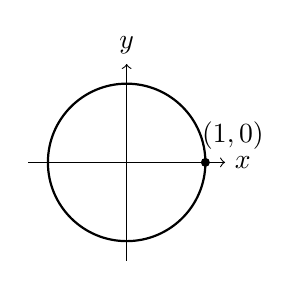
\begin{tikzpicture}
        \draw[thick] (0cm, 0cm) circle(1cm);
        \draw[->] (0,-1.25cm) -- (0,1.25cm) node[above] {$y$};
        \draw[->] (-1.25,0) -- (1.25cm,0) node[right] {$x$};
        \filldraw[black] (1cm, 0) circle(1.4pt);
        \draw (1.35cm,0cm) node[above=1pt] {$(1,0)$};
    \end{tikzpicture}
    \caption{Illustration of the unit circle, on which we place all convolution
    eigenvalues $\phi = x + iy$.}
\end{figure}
For the equivalent one convolution network. We therefore claim that adding convolutions to this kind of eigenspace normalized linear network will add additional degrees of freedom to eigenspace rotations around the unit circle. Having set all $r_{m,n} = 1$ we claim to run a more stable network, because we only rotate, but do not rescale with additional layers.
This convolution should remain stable when added to the  recurrent convLSTM state update equation. \\
However to apply this idea to convNets in space the non-linearity needs to be taken care of.

\subsubsection{Network conditioning}
In linear algebra when solving $A\mathbf{x} = b$ or $\min_x \| Ax - b\|$ an important property
is the condition number. It is a measure of the solutions sensitivity to small perturbations in $\mathbf{x}$. A problem is considered to be ill conditioned when $A$'s assiciated condition number is very large. 
A problem's conditioning is measured using:
\begin{align}
\kappa = \text{max}_{i,j}| \dfrac{\phi_i}{\phi_j}|
\end{align}
In other words the matrix condition $\kappa$ is the norm of the ratio of the largest and smallest eigenvalue. By enforcing $\| \phi \| = 1$ we also ensure a constant condition number of one for our convolution matrices. We hope to increase overall network stability this way, because our convolutions should not react very sensitively to small input perturbations.

\subsection{Two dimensional convolutions}
Discrete convolution is often described as sliding a kernel over an image. This operation may be expressed in terms of matrix-vector multiplication. For example the two dimensional convolution:
\begin{align}
A * B =
\begin{pmatrix}
a_1 & a_2 \\
a_3 & a_4
\end{pmatrix}
*
\begin{pmatrix}
b_1 & b_2 \\
b_3 & b_4
\end{pmatrix}
\end{align}
May be expressed using matrix multiplication as:
\begin{align}
A*B = K^T \cdot B_{\text{flat}}
\end{align}
Where $b_{\text{flat}}$ is a vector constructed by concatenation of B's rows.
And the matrix K defined as:
\begin{align} K =
\begin{pmatrix}
a_1 & a_2 & 0 & a_3 & a_4 & 0   & 0 & 0 &   0 \\
0   & a_1 & a_2 & 0 & a_3 & a_4 & 0 & 0 &   0 \\
0   & 0 & 0 & a_1 & a_2 & 0 & a_3 & a_4 &   0 \\
0   & 0 & 0 & 0   & a_1 & a_2 & 0 & a_3 & a_4 \\
\end{pmatrix}
\end{align}
Matrix $K$, describes a convolution, but is not circulant. 

\subsubsection{Doubly block circulant matrices}
\begin{figure}
\input{img/Kt.tex}
% This file was created by matplotlib2tikz v0.6.15.
\begin{tikzpicture}

\begin{axis}[
hide x axis,
hide y axis,
xmin=-0.5, xmax=15.5,
ymin=-0.5, ymax=15.5,
tick align=outside,
tick pos=left,
x grid style={white!69.01960784313725!black},
y grid style={white!69.01960784313725!black}
]
\addplot graphics [includegraphics cmd=\pgfimage,xmin=-0.5, xmax=3.5, ymin=8.5, ymax=-0.5] {./img/2dcirc1.png};
\addplot graphics [includegraphics cmd=\pgfimage,xmin=-0.5, xmax=15.5, ymin=15.5, ymax=-0.5] {./img/2dcirc2.png};
\end{axis}

\end{tikzpicture}
\caption{Visualization of a two dimensional convolution matrix and its square doubly circulant cousin.}
\label{fig:2dconv}
\end{figure}
In order to turn the convolution matrix into a square doubly circulant matrix, padding is required in both kernel and target matrix. A doubly circulant matrix is a block matrix consisting out of circulant blocks which are arranged in a circular pattern. In order to obtain circulant blocks the circular pattern must be finished, which is why the resulting matrix will be square by definition.
Padding $A$ and $B$ leads to\footnote{I think its probably possible to come up with a less wasteful way to do the padding i.e. remove the second zero row and column.}:
\begin{align}
A_p = \begin{pmatrix}
a_1 & a_2 & 0 & 0 \\
a_3 & a_4 & 0 & 0 \\
0 & 0 & 0 & 0 \\
0 & 0 & 0 & 0 \\
\end{pmatrix}
B_p = \begin{pmatrix}
b_1 & b_2 & 0 & 0 \\
b_3 & b_4 & 0 & 0 \\
0 & 0 & 0 & 0 \\
0 & 0 & 0 & 0 \\
\end{pmatrix}
\end{align}
In this case the circular convolution matrix can be set up according to:
\begin{align}
C_0 &= circ(c_0) = \begin{pmatrix} a_1 & a_2 & 0 & 0 \end{pmatrix} \\
C_1 &= circ(c_1) = \begin{pmatrix} a_2 & a_3 & 0 & 0 \end{pmatrix} \\
C_2 &= circ(c_2) = \begin{pmatrix} 0 & 0 & 0 & 0 \end{pmatrix} \\
C_3 &= circ(c_3) = \begin{pmatrix} 0 & 0 & 0 & 0 \end{pmatrix} \\
\end{align}
Which leads to the resulting matrix $C$:
\begin{align}
C_b = \begin{pmatrix} C_0 & C_1 & C_2 & C_3 \\
                    C_3 & C_0 & C_1 & C_2 \\
                    C_2 & C_3 & C_0 & C_2 \\
                    C_1 & C_2 & C_3 & C_0 \\
    \end{pmatrix}
\end{align}
A visualization of this matrix is shown in figure~\ref{fig:2dconv} on the right. Multiplication of $C_b \cdot B_{p\text{ flat}}$ will lead to a zero padded version of $K^T \cdot B_{\text{flat}}$.


\subsubsection{Doubly block circulant matrices and their eigenvalues}
\begin{figure}
\centering
\input{img/2dcircfreq.tex}
\caption{Absolute values of complex doubly block circulant matrix constructed in the frequency domain.}
\end{figure}

In order to be able to enforce $\| \phi \| = 1$. We would like to be able to construct doubly block circulant matrices in their eigenspace. According to \cite[page 185]{Davis}, their diagonalization is given by:
\begin{align} 
C_b = \overline{(F_m \otimes F_n)^T} \Lambda (F_m \otimes F_n)
\label{eq:dc_spec}
\end{align}
$F_m$ and $F_n$ denote fourier matrices. $\Lambda$ has complex eigenvalues sitting on its diagonal. Their choice determines the block structure of the resulting 
matrix, which will be square with $m$ block containing $n$ rows each.
Given a real input matrix we can find Lambda from:
\begin{align}
\Lambda = (F_m \otimes F_n) C_b \overline{(F_m \otimes F_n)^T}
\end{align}
We believe that~\ref{eq:dc_spec} is differentiable and should enable use to construct and optimize doubly block circulant matrices in the frequency domain. In order to ensure a real valued output $\Lambda$ must be symmetric with respect to the real axis.

\subsubsection{The spectrum of real doubly block circulant matrices.}
Tricky because doubly block circulants are not also circulant. So we cannot simply apply the one dimensional insight gained from working with circulants to block circulants. However block circulant spectra are point-symmetric in tow dimensions. Figures~\ref{fig:circ_spec2d} and~\ref{fig:block_circ_spec2d} illustrate this. The spectrum shown in ~\ref{fig:circ_spec2d} is symmetric along the a-Axis, when cutting after its third element and disregarding the first eigen-vale. The block circulant case shown in ~\ref{fig:circ_spec2d}, we find the same symmetry in the zeroth column and 4th row. The middle block is point symmetric. 

\begin{figure}
\centering
% This file was created by matplotlib2tikz v0.6.15.
\begin{tikzpicture}

\begin{axis}[
hide x axis,
hide y axis,
xmin=-0.5, xmax=3.5,
ymin=-0.5, ymax=3.5,
tick align=outside,
tick pos=left,
x grid style={white!69.01960784313725!black},
y grid style={white!69.01960784313725!black}
]
\addplot graphics [includegraphics cmd=\pgfimage,xmin=-0.5, xmax=3.5, ymin=3.5, ymax=-0.5] {./img/circ1.png};
\addplot graphics [includegraphics cmd=\pgfimage,xmin=-0.5, xmax=3.5, ymin=3.5, ymax=-0.5] {./img/circ2.png};
\end{axis}

\end{tikzpicture}
% % This file was created by matplotlib2tikz v0.6.15.
\begin{tikzpicture}

\definecolor{color0}{rgb}{0.12156862745098,0.466666666666667,0.705882352941177}

\begin{groupplot}[group style={group size=2 by 2, vertical sep=50pt, horizontal sep=70pt}]
\nextgroupplot[
xmin=-0.5, xmax=15.5,
ymin=-0.5, ymax=15.5,
tick align=inside,
tick pos=left,
x grid style={white!69.01960784313725!black},
y grid style={white!69.01960784313725!black},
xlabel={x-index},
ylabel={y-index},
height=0.5\linewidth,
width=0.5\linewidth
]
\addplot graphics [includegraphics cmd=\pgfimage,xmin=-0.5, xmax=15.5, ymin=15.5, ymax=-0.5] {./img/denseCirc1.png};
\nextgroupplot[
xmin=-40.4226209677419, xmax=144.422620967742,
ymin=-35.2089285714286, ymax=35.2089285714286,
tick align=inside,
tick pos=left,
x grid style={white!69.01960784313725!black},
y grid style={white!69.01960784313725!black},
xlabel={real-part},
ylabel={imaginary-part},
height=0.1\linewidth,
width=0.5\linewidth
]
\addplot [only marks, draw=color0, fill=color0, colormap/viridis]
table{%
x                      y
+1.360000000000000e+02 +0.000000000000000e+00
-8.000000000000000e+00 -7.999999999999998e+00
-8.000000000000000e+00 -1.972152263052530e-31
-8.000000000000000e+00 +8.000000000000000e+00
-3.200000000000000e+01 -3.200000000000000e+01
+2.220446049250312e-16 -1.387778780781451e-17
-5.551115123125783e-17 -5.551115123125804e-17
+7.632783294297885e-17 +1.665334536937729e-16
-3.200000000000000e+01 +1.577721810442024e-30
+1.249000902703300e-16 -8.326672684688689e-17
-1.499759782661856e-31 -2.711709361697228e-31
-2.775557561562941e-17 -1.665334536937735e-16
-3.199999999999999e+01 +3.200000000000001e+01
-1.526556658859594e-16 +2.359223927328457e-16
-5.551115123125800e-17 -1.110223024625156e-16
+6.245004513516419e-17 +1.526556658859599e-16
};
\nextgroupplot[
xmin=-0.75, xmax=15.75,
ymin=-40.4, ymax=144.4,
tick align=inside,
tick pos=left,
x grid style={white!69.01960784313725!black},
y grid style={white!69.01960784313725!black},
xlabel={position on diag$(\Lambda)$},
ylabel={real-part},
height=0.1\linewidth,
width=0.5\linewidth 
]
\addplot [semithick, color0, forget plot]
table {%
0 136
1 -8
2 -8
3 -8
4 -32
5 2.22044604925031e-16
6 -5.55111512312578e-17
7 7.63278329429788e-17
8 -32
9 1.2490009027033e-16
10 -1.49975978266186e-31
11 -2.77555756156294e-17
12 -32
13 -1.52655665885959e-16
14 -5.5511151231258e-17
15 6.24500451351642e-17
};
\nextgroupplot[
xmin=-0.75, xmax=15.75,
ymin=-35.2, ymax=35.2,
tick align=inside,
tick pos=left,
x grid style={white!69.01960784313725!black},
y grid style={white!69.01960784313725!black},
xlabel={position on diag$(\Lambda)$},
ylabel={imaginary-part},
height=0.1\linewidth,
width=0.5\linewidth
]
\addplot [semithick, color0, forget plot]
table {%
0 0
1 -8
2 -1.97215226305253e-31
3 8
4 -32
5 -1.38777878078145e-17
6 -5.5511151231258e-17
7 1.66533453693773e-16
8 1.57772181044202e-30
9 -8.32667268468869e-17
10 -2.71170936169723e-31
11 -1.66533453693773e-16
12 32
13 2.35922392732846e-16
14 -1.11022302462516e-16
15 1.5265566588596e-16
};
\end{groupplot}

\end{tikzpicture}
\caption{Circulant matrix pattern and spectrum.}
\label{fig:circ_spec2d}
\end{figure} 

\begin{figure}
% % This file was created by matplotlib2tikz v0.6.15.
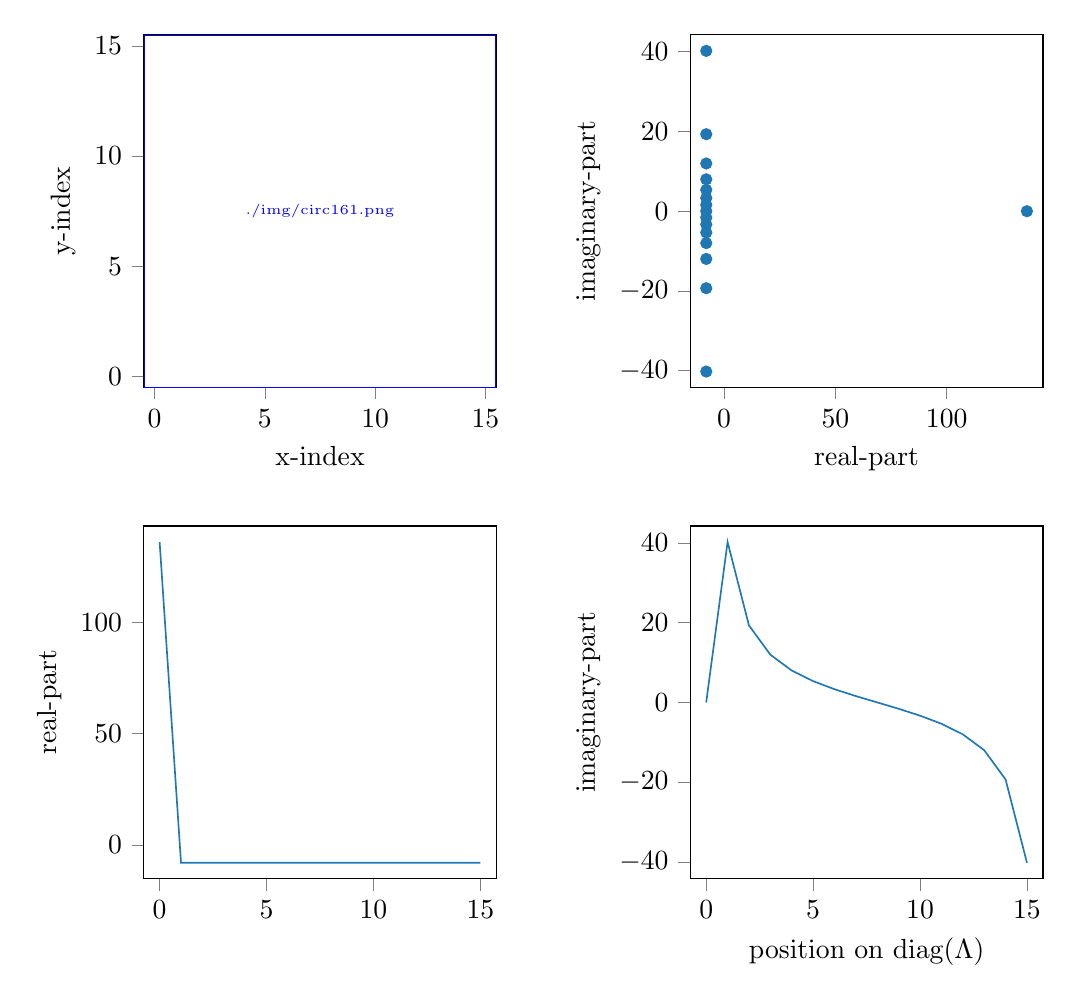
\begin{tikzpicture}

\definecolor{color0}{rgb}{0.12156862745098,0.466666666666667,0.705882352941177}

\begin{groupplot}[group style={group size=2 by 2, vertical sep=50pt, horizontal sep=70pt}]
\nextgroupplot[
xmin=-0.5, xmax=15.5,
ymin=-0.5, ymax=15.5,
tick align=outside,
tick pos=left,
x grid style={white!69.01960784313725!black},
y grid style={white!69.01960784313725!black},
xlabel={x-index},
ylabel={y-index},
height=0.5\linewidth,
width=0.5\linewidth
]
\addplot graphics [includegraphics cmd=\pgfimage,xmin=-0.5, xmax=15.5, ymin=15.5, ymax=-0.5] {./img/circ161.png};
\nextgroupplot[
xmin=-15.2306048387097, xmax=143.23060483871,
ymin=-44.249516102136, ymax=44.249516102136,
tick align=outside,
tick pos=left,
x grid style={white!69.01960784313725!black},
y grid style={white!69.01960784313725!black},
xlabel={real-part},
ylabel={imaginary-part},
height=0.5\linewidth,
width=0.5\linewidth
]
\addplot [only marks, draw=color0, fill=color0, colormap/viridis]
table{%
x                      y
+1.360000000000000e+02 +0.000000000000000e+00
-7.999999999999987e+00 +4.021871593700678e+01
-7.999999999999985e+00 +1.931370849898476e+01
-7.999999999999974e+00 +1.197284610132390e+01
-8.000000000000000e+00 +8.000000000000000e+00
-8.000000000000000e+00 +5.345429103354396e+00
-7.999999999999998e+00 +3.313708498984765e+00
-7.999999999999986e+00 +1.591298939037273e+00
-8.000000000000000e+00 +0.000000000000000e+00
-8.000000000000004e+00 -1.591298939037262e+00
-8.000000000000004e+00 -3.313708498984756e+00
-7.999999999999999e+00 -5.345429103354377e+00
-8.000000000000000e+00 -8.000000000000000e+00
-8.000000000000007e+00 -1.197284610132392e+01
-8.000000000000016e+00 -1.931370849898477e+01
-8.000000000000043e+00 -4.021871593700679e+01
};
\nextgroupplot[
xmin=-0.75, xmax=15.75,
ymin=-15.2, ymax=143.2,
tick align=outside,
tick pos=left,
x grid style={white!69.01960784313725!black},
y grid style={white!69.01960784313725!black},
ylabel={real-part},
height=0.5\linewidth,
width=0.5\linewidth 
]
\addplot [semithick, color0, forget plot]
table {%
0 136
1 -7.99999999999999
2 -7.99999999999998
3 -7.99999999999997
4 -8
5 -8
6 -8
7 -7.99999999999999
8 -8
9 -8
10 -8
11 -8
12 -8
13 -8.00000000000001
14 -8.00000000000002
15 -8.00000000000004
};
\nextgroupplot[
xmin=-0.75, xmax=15.75,
ymin=-44.2405875307075, ymax=44.2405875307075,
tick align=outside,
tick pos=left,
x grid style={white!69.01960784313725!black},
y grid style={white!69.01960784313725!black},
xlabel={position on diag$(\Lambda)$},
ylabel={imaginary-part},
height=0.5\linewidth,
width=0.5\linewidth
]
]
\addplot [semithick, color0, forget plot]
table {%
0 0
1 40.2187159370068
2 19.3137084989848
3 11.9728461013239
4 8
5 5.3454291033544
6 3.31370849898476
7 1.59129893903727
8 0
9 -1.59129893903726
10 -3.31370849898476
11 -5.34542910335438
12 -8
13 -11.9728461013239
14 -19.3137084989848
15 -40.2187159370068
};
\end{groupplot}

\end{tikzpicture}
% This file was created by matplotlib2tikz v0.6.15.
\begin{tikzpicture}

\begin{axis}[
hide x axis,
hide y axis,
xmin=-0.5, xmax=15.5,
ymin=-0.5, ymax=15.5,
tick align=outside,
tick pos=left,
x grid style={white!69.01960784313725!black},
y grid style={white!69.01960784313725!black}
]
\addplot graphics [includegraphics cmd=\pgfimage,xmin=-0.5, xmax=3.5, ymin=8.5, ymax=-0.5] {./img/2dcirc1.png};
\addplot graphics [includegraphics cmd=\pgfimage,xmin=-0.5, xmax=15.5, ymin=15.5, ymax=-0.5] {./img/2dcirc2.png};
\end{axis}

\end{tikzpicture}
\caption{Block Circulant matrix pattern and spectrum.}
\label{fig:block_circ_spec2d}
\end{figure}

\section{Other related ideas}
\subsection{Rotation-GRU in $\mathbb{R}$}
This section proposes the rotation-GRU, a modified version of the conv-GRU, which builds on the theory above. Recall the conv-GRU definition:
\begin{align}
Z_t &= \sigma(W_{xz} * X_t + W_{hz} * H_{t-1} + b_z), \\
R_t &= \sigma(W_{xr} * X_t + W_{hr} * H_{t-1} + b_r), \\
H_t' &= f(W_{xr} * X_t) + R_t \circ (W_{hp} * H_{t-1}), \\
H_t &= (1 - Z_t) \circ H_t' + Z_t \circ H_{t-1}.
\end{align}
When optimizing the convolutions, while enforcing $\| \phi \| = 1$, 
changing the state update equation $H_t$ to:
\begin{align}
H_t &= W_h * ((1 - Z_t) \circ H_t' + Z_t \circ H_{t-1}).
\end{align}
Assuming that the gates $Z_t$ and $R_t$ keep the absolute value of 
$((1 - Z_t) \circ H_t' + Z_t \circ H_{t-1})$ under control, like they learn to
do in the standard conv-GRU case, the network should remain stable, because the eigenvalues of $W_h$ are normalized. A rational similar to the one in section~\ref{seq:linstab} should hold.

\subsubsection{Gradients of the Rotation-GRU}
So far we have only considered the forward pass of the optimization process. In order for our ideas to work we must also consider the backward pass. The two are similar, because in time, input and error flow follow the dynamics of the state equation $H_t$. This section examines the gradient equations for the convGRU and rotationGRU in detail. \dots ..TODO!

\bibliographystyle{plain}
\bibliography{literature}
% \begin{thebibliography}{9}
% \bibitem[Goodfellow]{goodfellow} \emph{Deep Learning},
% MIT Press 2017
% \bibitem[Strang]{strang} \emph{Linear algebra},
% MIT Press 2006
% \bibitem[Gray]{gray} \emph{Toeplitz and Circulant Matrices: A Review},
% now publishing
% \bibitem[Bronstein]{Bronstein} \emph{Springer Taschenbuch der Mathematik}, Springer Spektrum
% % \bibitem[Gers et al]{Gers} \emph{Learning to Forget: Continual Prediction with LSTM}
% \bibitem[Davis]{Davis} \emph{Circulant Matrices}, John Wiley and Sons
% \bibitem[Pascanu]{Pascanu} \emph{On the difficulty of training Recurrent Neural networks}, \url{https://arxiv.org/pdf/1211.5063.pdf}
% \bibitem[Arjovsky]{Arjovsky} \emph{Unitary Evolution Recurrent Neural networks.}
% \bibitem[Briggs]{Briggs} \emph{The DFT, an Owners Manual for the Discrete Fourier Transform.}
% \bibitem[Bornemann]{Bornemann} \emph{Funktionentheorie}, \url{http://www.springer.com/de/book/9783034804721}
% \bibitem[Trabelsi]{Trabelsi} \emph{Deep Complex Networks}, ICLR 2018 \url{https://arxiv.org/pdf/1705.09792.pdf}
% \bibitem[Hyland]{Hyland}, \emph{Learning Unitary Operators with Help From u (n).}, aaai 2017, \url{http://www.aaai.org/ocs/index.php/AAAI/AAAI17/paper/download/14930/14373}
% \bibitem[Guberman]{Guberman} \emph{On Complex Valued Convolutional Neural Networks}, \url{https://arxiv.org/pdf/1602.09046.pdf}
% \bibitem[Wisdom]{Wisdom} \emph{Full-Capacity Unitary Recurrent Neural Networks}, \url{https://arxiv.org/abs/1611.00035}
% \bibitem[Jing]{Jing} \emph{Gated Orthogonal Recurrent Units: On Learning to Forget}, \url{https://arxiv.org/pdf/1706.02761.pdf}
% \bibitem[Trabelsi]{Trabelsi} \emph{Deep Complex Networks}, \url{https://arxiv.org/pdf/1705.09792.pdf}
% \bibitem[Freeman]{Freeman} \emph{The Design and Use of Steerable Filters}, \url{http://people.csail.mit.edu/billf/www/papers/steerpaper91FreemanAdelson.pdf}
% \bibitem[Michaelis]{Michaelis} \emph{A lie group approach to steerable filters}, \url{https://www.sciencedirect.com/science/article/pii/016786559500066P?via%3Dihub}
% \bibitem[Virtue]{Virtue} \emph{BETTER THAN REAL: COMPLEX-VALUED NEURAL NETS FOR MRI FINGERPRINTING}, \url{https://arxiv.org/pdf/1707.00070.pdf}
% \bibitem[Scardapane]{Scardapane}, \emph{Complex-valued Neural Networks with Non-parametric Activation Functions}, \url{https://arxiv.org/pdf/1802.08026.pdf}
% \end{thebibliography}

\end{document}